\renewcommand{\chaptername}{Introduction}
\chapter*{Introduction}
\setcounter{page}{1}
\pagenumbering{arabic}
\addcontentsline{toc}{chapter}{Introduction}


\shorthandoff{-} 

\section{Taxonomy and characteristics of \tax{Escherichia coli}}
\hspace*{0,5cm} Domain: \hspace{0,5cm} \tax{Bacteria}\\%
\hspace*{1,5cm} Phylum: \hspace{0,5cm} \tax{Proteobacteria}\\%
\hspace*{2,5cm} Class: \hspace{0,5cm} \tax{Gammaproteobacteria}\\%
\hspace*{3,5cm} Order: \hspace{0,5cm} \tax{Enterobacteriales}\\%
\hspace*{4,5cm} Family: \hspace{0,5cm} \tax{Enterobacteriaceae}\\%

\tax{E. coli} is Gram-negative bacterium with facultative anaerobic metabolism.
Since its first isolation from infant faeces by Theodor Escherich in 1885 \cite{friedmann2006escherich}, this organism was found in gastrointestinal tract of other warm-blooded animals and reptiles \cite{gopee2000longitudinal} as well as in environmental samples such as soil or water.
\tax{E. coli} is known to be a part of normal intestine microbiota.
On the other hand extraintestinal infections caused by this bacterium are common and some strains (e.g. STEC) even possess virulence factors leading to heavy intestinal infections when expressed \cite{allocati2013escherichia}.


Although the presence of \tax{E. coli} in water is still widely used as an indicator of fecal contamination recent studies show that some \tax{E. coli} isolates are able to  reproduce in soil \cite{byappanahalli2004indigenous, somorin2016general}.
Moreover strains inhabiting soil for a long time were found to be distinctive \cite{walk2009cryptic, walk2015cryptic}.
This raises the questions how these bacteria survive outside their hosts and how do they evolve under such conditions.

\section{Transcription and memory}
A bacterial genome consists of hundreds and thousands of genes, but not all of them are active at all the time.
Gene expression changes during a cell cycle, when a nutrient source is altered or if surrounding conditions begin to be unfavourable.
It is vital for a living cell to sense what is happening in the environment it is present at and react accordingly by transcription initiation or silencing of appropriate genes.
Some studies has shown that cells with the same genetic background might react differently or at a different rate to the same stimulus based on their and their ancestors recent experience \cite{mathis2017asymmetric, ronin2017long}.
Such ability is advantageous especially if the change in the conditions is predictable and repeats periodically.

\subsection{Epigenetic mechanisms in bacteria}
Epigenetics is understood as a heritable change in gene expression without simultaneous changes in DNA primary sequence.
Various epigenetic mechanisms such as histone modifications, genomic imprinting or RNA associated silencing are well studied in eukaryotes \cite{durso2014mechanisms}.
In bacterial domain DNA methylation by methyltransferases is mostly mentioned, although positive and double negative feedback loops play their role as well especially in terms of population bistability \cite{casadesus2006epigenetic, casadesus2013programmed, adhikari2016dna}.

\subsubsection{DNA methylation by orphan methyltransferases}
Orphan methyltransferases (MTs) were initially studied within restriction-modification system as a bacterial defence against phages, although Dam's ability to alter some gene expression was already described in mid-80s \cite{sternberg1985evidence, bickle1993biology}.
As orphan MTs lack their cognate restriction endonucleases their role in bacterial cells is not as a primitive immune system, but among others can act as a transcription regulators.
I describe the epigenetic mechanisms of Dam in detail below as the MT whose relationship to cell memory is most understood.
Some authors consider the change in expression of certain genes in \tax{Caulobacter crescentus} which is associated with an orphan MT called CcrM to be epigenetic as well \cite{casadesus2006epigenetic, adhikari2016dna}.
However I do not include it here as these transcriptional changes are not heritable and occur only during a part of cell cycle.
Other \tax{E. coli} orhan MTs are mentioned briefly as well although none of them is known to play a role in epigenetics so far.

\textbf{Dam}, one of two first orphan MTs described in \tax{E. coli}, methylates adenine in 5'-GATC-3' sequences to N$^6$-methyladenine (6mA) \cite{marinus1973isolation}.
Its homologs were found in some bacteriophages as well as in other \tax{Gammaproteobacteria}, however many of bacterial DNA adenine methylases are associated with restriction endonucleases \cite{low2001roles, casadesus2006epigenetic, bochow2012bacteriophage}.
On the other hand strains having an orphan DNA adenine methylase can be characterized by presence of SeqA and MutH, overrepresentation of GATC sites in \tax{oriC}, genes close to it and in the \tax{dnaA} promoter \cite{sobetzko2016distamo}.
For most of the DNA both strands of chromosome are fully methylated throughout the cell cycle if Dam is present.
Of course, one of the exceptions is a short time hemimethylation of a leading strand and Okazaki fragments right after their synthesis during replication.
Both strands lack GATC methylation in \tax{dam} mutants, moreover higher mutation rate, uncoordinated replication initiation or loss of virulence were observed as well.
Interestingly for some species e.g. \tax{Vibrio cholerae} the presence of an orphan DNA adenine methylase is vital, whereas it is non-essential for other, such as \tax{E. coli} \cite{casadesus2006epigenetic, casadesus2013programmed, adhikari2016dna}.

As implied above several GATC sites escape Dam methylation.
This happens if another regulatory protein recognises a specific DNA biding site which overlaps GATC sequence and thus competes with Dam for it \cite{correnti2002dam}.
Such mechanism leading to epigenetic switch is well characterized in synthesis of \tax{pap} pili in uropathogenic \tax{E. coli} (UPEC) \cite{peterson2008competitive}.
The regulatory sequence of the \tax{pap} operon contains two sets of Lrp binding sites 1-3 and 4-6.
In both of them GATC sequence is present, GATC$^{prox}$ within site 2 and GATC$^{dist}$ within site 5 (Fig.~\ref{pap}) \cite{blyn1990regulation}.
\begin{figure}[t!]
  \centering
  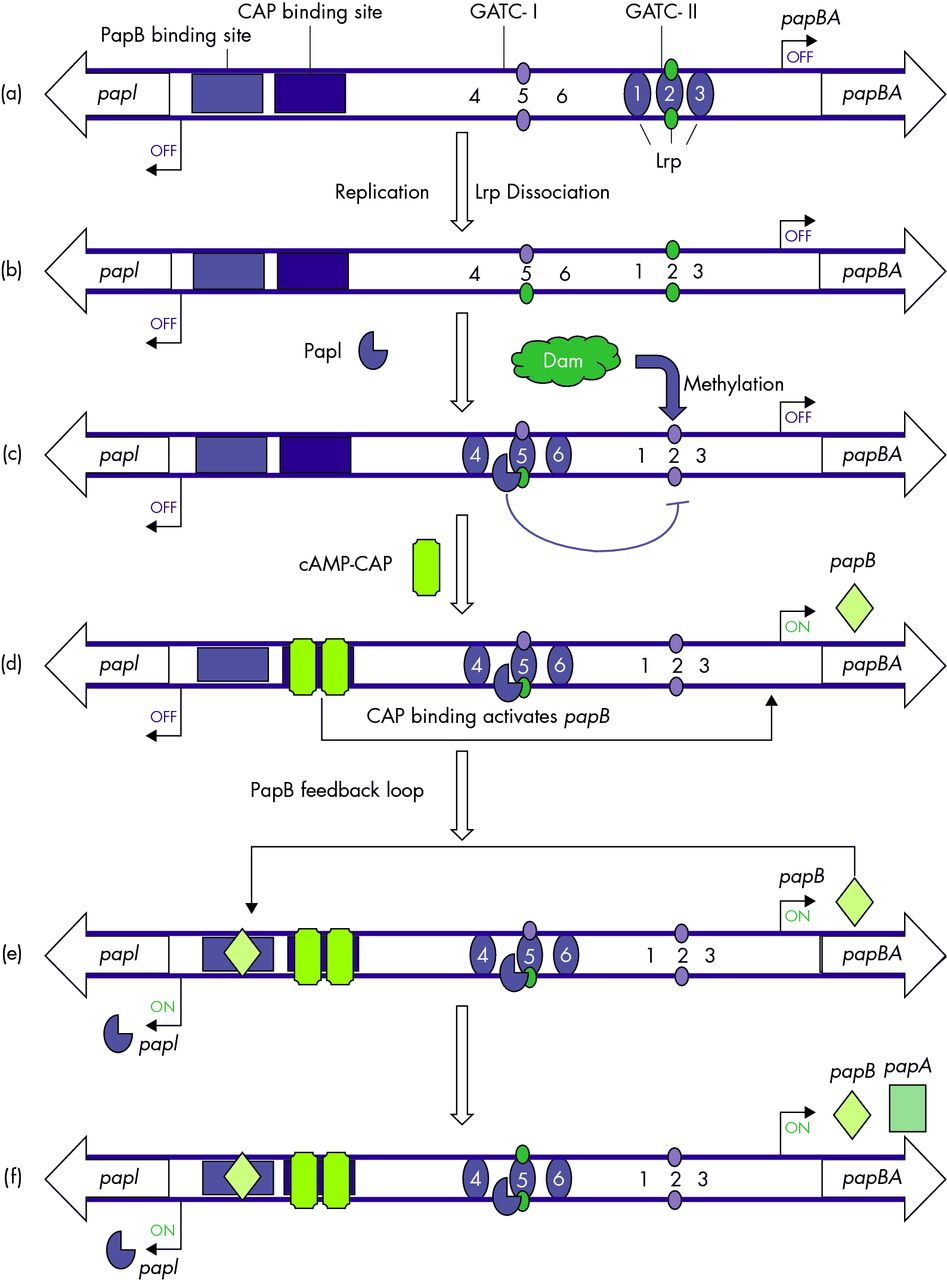
\includegraphics[scale=1.5]{text/Pictures/papPili.jpeg}
	\caption{Model of the \tax{pap} phase OFF to ON switch. GATC$^{dist}$ and GATC$^{prox}$ are represented by GATC-I and GATC-II, respectivelly. (reproduced from \cite{adhikari2016dna})}
	\label{pap}
\end{figure}
During the OFF phase \tax{pap} pili are not produced because Lrp occupies GATC$^{prox}$ site which remains nonmethylated on both strands while GATC$^{dist}$ is fully methylated.
Lrp in this position prevents binding not only by Dam but by $\sigma^{70}$ RNA polymerase as well inhibiting expression of \tax{papBA} gene \cite{weyand2000regulation}.
For switch to ON phase an initial Lrp dissociation from sites 1-3 is necessary.
This likely happens during replication when an opportunity for Lrp to bind the hemimethylated GATC$^{dist}$ site instead of GATC$^{prox}$ raises.
The probability of this switch depends on the level of regulatory protein PapI in the cell as complex PapI/Lrp has lower affinity to site 2 but binds more likely to hemimethylated sites 4-6 than to fully methylated DNA \cite{hernday2003mechanism}.
Besides Lrp release from GATC$^{prox}$ site enables access of Dam to it so it can become methylated which further reduces Lrp affinity to 1-3 sites.
Even though RNA polymerase's access to \tax{papBA} promoter is not blocked any more the expression itself requires cAMP-CAP binding (Fig \ref{pap}\textcolor{red}{d}) \cite{weyand2001essential}.
When PapB is beeing produced it acts as a \tax{papI} gene transcription activator leading to a feedback loop which stabilizes the cells in ON phase \cite{forsman1989autoregulation}.
However the described transition from OFF to ON phase occurs with 100-fold lower frequency than vice versa \cite{blyn1990regulation}.
The process of this opposite transition i.e. from ON to OFF phase involves transfer of Lrp from GATC$^{dist}$ to GATC$^{prox}$ during replication but the exact mechanism is not fully understood yet \cite{adhikari2016dna}.

Another well known orphan MT in \tax{E. coli} is \textbf{Dcm} which methylates second cytosine in 5'-CC(A/T)GG-3' motif to 5-methylcytosine (5mC) \cite{marinus1973isolation}.
Even though neither this one is necessary for \tax{E. coli} survival and some strains were found lacking \tax{dcm} gene, link between certain genes expression and presence of this MT was described.
Dcm seems to slow down expression of ribosomal genes \tax{rplC} and \tax{rpsJ} and inhibit transcription of \tax{sugE} gene connected with higher antimicrobial resistance \cite{militello2012conservation, militello2014cytosine}.
Both is happening predominantly during early stationary phase.
Next study shows increased expression of stress response sigma factor RpoS in \tax{dcm} mutant \cite{kahramanoglou2012genomics}.
Recently additional 63 genes were discovered to be affected if Dcm activity is inhibited \cite{militello20165}.
Most of these genes are up-regulater during early stationary phase if methylation by Dcm is silenced.

Lastly \textbf{YhdJ} is an orphan MT methylating 3' adenine of 5'-ATGCAT-3' sequence to 6mA when overexpressed.
Deleting \tax{yhdJ} gene produces neither loss of viability of \tax{E. coli} nor changes in its phenotype.
In addition, the expression of the gene is very low under usual laboratory conditions and nothing is known about transcription regulation of the gene \cite{broadbent2007yhdj}.

\subsubsection{Feedback loops}
System where a product is able to affect positively or negatively its own production is called a feedback loop.
The influence of the output on itself might be direct or indirect if multiple effectors are involved.
Feedback loops are quite common in bacterial gene regulation and can lead to epigenetic switches \cite{smits2006phenotypic, veening2008bistability}.
Positive feedback loop and double negative feedback loop are known to play a role in memory of prokaryotes so far and are characterized in detail below.

\textbf{Positive feedback loop} is the first described example of bacterial epigenetics.
It was shown already in 1957 that \tax{E. coli} sub-population primed by high concentration of lactose analogue TMG is able to maintain \tax{lac} operon fully induced even in low non-inducible TMG concentrations \cite{novick1957enzyme}.
While if the same bacteria are exposed to the low non-inducible TMG concentration without priming the \tax{lac} operon remains repressed by LacI.
The mechanism behind this resides in different levels of $\beta$-galactoside permease (LacY) in TMG induced and naive cells.
Induced population has high level of the permease present in membrane as \tax{lacY} gene expression is activated by high TMG concentrations.
This state is preserved in a sub-population of induced cells after transfer into low TMG concentration as the abundant permease is able to maintain intracellular TMG level high enough to avoid LacI repression.
Thus the high level of permease leads to high intracellular TMG concentration which in turn acts as permease transcription activator.
On the other side naive cells have very small amounts of LacY if any thus they are not able to obtain TMG from the solution to activate \tax{lac} operon expression \cite{smits2006phenotypic, casadesus2013programmed}.

Another nice example of a long-term virulence epigenetic switch mediated by a positive feedback loop was published last year.
Enteropathogenic \tax{E. coli} (EPEC) coexists in two, non-virulent and hyper-virulent, sub-populations during growth \cite{ronin2017long}.
This bimodality was first observed  using ScanLag \cite{levin2014scanlag} as a difference in growth rates of the two groups resulting in BIG and SMALL colony morphotypes, for early and late appearing colonies, respectively.
In transcription level it is a change in \tax{per} operon expression (located on EAF plasmid) and \tax{per} regulated genes.
EPEC cultivation in virulence-activating conditions gives rise to \tax{per}-ON hyper-virulent aggregative sub-population (SMALL phenotype) reaching nearly 100\% \cite{ronin2017long}.
Interestingly this high ratio of \tax{per}-ON vs \tax{per}-OFF cells remains for many generations even after transferring the culture back into non-activating conditions, although naive EPEC culture contains only a minority of \tax{per}-ON cells.
Transition back from \tax{per}-ON to \tax{per}-OFF phase is achieved when cells are grown up to stationary phase.
The long-term stability of \tax{per}-ON state relies on a positive feedback of PerA which acts as activator of its own gene beside \tax{perB} and \tax{perC} in \tax{per} operon (Fig.~\ref{per}) \cite{ibarra2003identification, ronin2017long}.
\begin{figure}[h!]
  \centering
  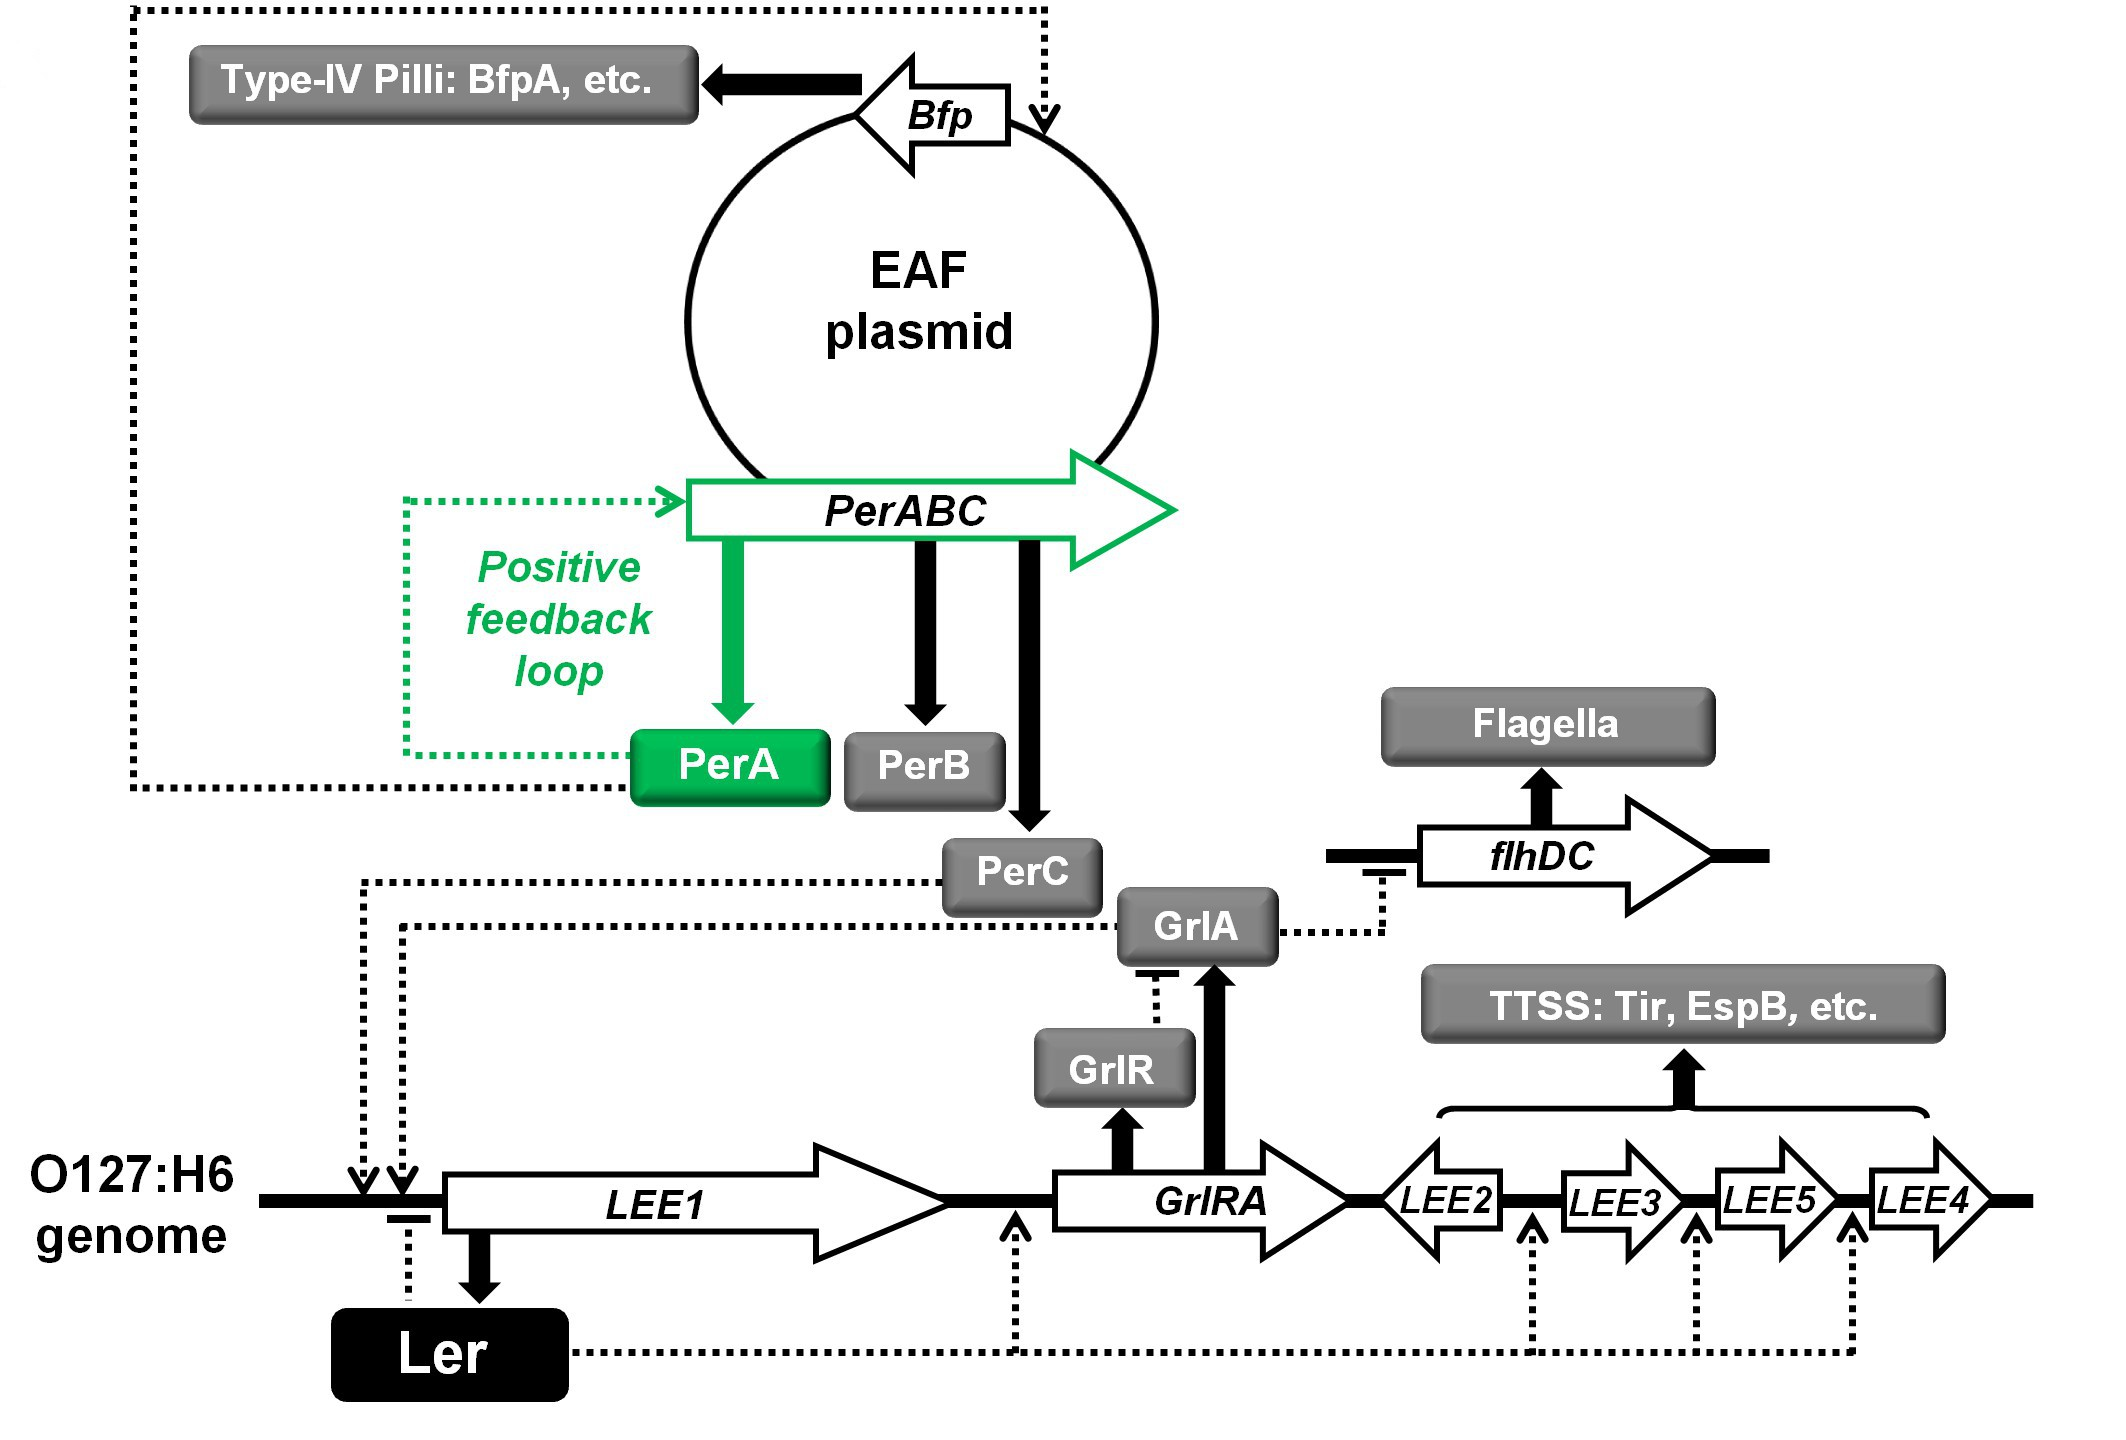
\includegraphics[scale=0.2]{text/Pictures/perOperonRegulation.jpg}
	\caption{Scheme of EPEC virulence regulation. PerA positivelly autoregulates \tax{perABC} operon and the triggers expression of type IV pili. PerC activates transcription of Ler which is the main regulator of T3SS secretion system machinery. (reproduced from \cite{ronin2017long})}
	\label{per}
\end{figure}



\cleardoublepage

